\section{System Architecture}
\subsection{Audited implementation and component boundaries}
The system snapshot is commit \code{f0e9d0d67422b0c286a2cb9e7d4e935a833a9533}, dated 9 November 2026, on \code{codex/social-master-plan-audit-remediation}. The local \code{main} revision is older and omits relevant remediations. The audited worktree was clean before the new paper artifacts were created. Source, analysis scripts, tests, JSON schemas, data snapshots, research documents, and reports are stored in distinct directories. Social is not currently distributed through a unified package or dependency lockfile. Entry points are Python modules and research scripts rather than a single comprehensive application command.

Figure~\ref{fig:architecture} shows the implemented composition. Platform collectors and case-specific preprocessing produce snapshots for legacy information analysis. A newer typed branch links source captures to an evidence ledger and bounded analysis. Video indexing and extraction form a separate local pipeline; the general incident runner does not automatically invoke the full media pipeline. The controller integrates a fixed Source Watch adapter and optional pretyped offline inputs. It does not dispatch every collector, autonomously expand source discovery, or infer every intermediate object from raw records.

\begin{figure}[tbp]
\centering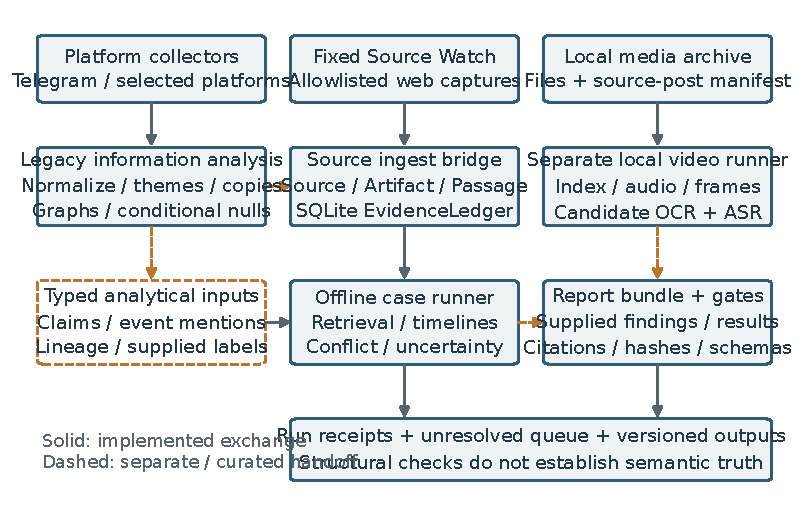
\includegraphics[width=\linewidth]{system_architecture.pdf}
\caption{Implemented Social components and integration boundaries at the audited revision. Solid arrows denote implemented exchanges; dashed arrows mark manual or separately executed adapters. The media and legacy-analysis branches are executable but are not all orchestrated by the general incident runner.}
\label{fig:architecture}
\end{figure}

\begin{table}[tbp]
\caption{System components: implementation and validation are separate dimensions. Paths are relative to the repository root; most analytical modules reside in \code{src/analysis/}.}
\label{tab:components}\small
\begin{tabularx}{\linewidth}{@{}p{25mm}X p{25mm}@{}}\toprule
Component & Concrete implementation and role & Evidence of readiness\\\midrule
Acquisition & \code{src/tg_collect.py}, \code{src/tg_comments_collect.py}, \code{src/source_watch_collect.py}; separate API/web collectors & Implemented; access-dependent, offline tests\\
Snapshot preparation & \code{build_continuation.py}, \code{prep.py}; verified merge and case relevance rules & Implemented; provenance checks; semantic relevance not independently validated\\
Information analysis & \code{analyze.py}, \code{coordination_lsh_audit.py}, \code{coordination_null_models.py} & Implemented; exact graph and bounded replay evaluated\\
Evidence accounting & \code{src/evidence_ledger.py}, \code{source_ingest_bridge.py}, \code{source_lineage.py} & Implemented; structural/reference tests\\
Evidence assessment & \code{claim_verification.py}; BM25, heuristics, aggregation & Retrieval implemented; semantic heuristics experimental\\
Events and conflict & \code{event_reconstruction.py}, \code{conflict_analysis.py}; supplied typed records & Implemented organization; physical truth not evaluated\\
Local media & \code{src/media_pipeline.py}, \code{video_pipeline_runner.py}, \code{media_fingerprints.py} & Implemented; technical receipts; semantic thresholds uncalibrated\\
Audience analytics & \code{audience_response.py}, \code{audience_aggregation.py} & Implemented contracts / aggregation; labels supplied, accuracy not evaluated\\
Workflow and reports & \code{offline_case_runner.py}, \code{incident_orchestrator.py}, \code{report_generator.py}, \code{evaluation_harness.py} & Bounded integration tested; end-to-end investigation not validated\\\bottomrule
\end{tabularx}
\end{table}

The distinction in Table~\ref{tab:components} is operationally important. Contract checks, append-only ledger insertion, and deterministic processors are reusable mechanisms. Claim inventories, selected passage bundles, physical-event intervals, and ASR reference strings in particular builders are curated research inputs. Dossier scripts format results; they do not independently verify every empirical statement they print. Platform schemas may declare a platform without supplying a native collector. None of these categories should be collapsed into a repository-wide production-readiness claim.

\subsection{Persistence and execution interfaces}
JSON and JSONL snapshots support streaming records and inspectable intermediate outputs. CSV serves graph edges, summaries, and selected evaluation tables. SQLite stores linked evidence records. Raw media and larger derivatives are maintained outside tracked source files, with manifests linking observations to bytes and derived text. PDF and Markdown are presentation outputs, not authoritative replacements for machine-readable results.

The reusable workflow accepts an \code{IncidentSpec}, explicit typed inputs, an output directory, and a producer Git revision. It records per-stage receipts and a run manifest. The caller must supply the true revision: recording a revision string does not prove that the executing source matched it. Budgets, cutoff times, path restrictions, bounded input sizes, and explicit \code{not_run} states constrain execution. This favors local inspectability and incremental use on a small research workstation over a distributed agent platform, while leaving substantial integration work at the collector-to-typed-record boundary.
